\chapter{Inference}
\thispagestyle{plain}
\label{ch:inference}

The trained \acrlong{cnn} model is deployed on the embedded system, where it is used to make prediction about new data.
This process is called inference.
% After training a \acrlong{cnn} model

% This chapter provides an overview of the inference application and describes the different components.
% This chapter provides an overview of the inference application and describes the camera library, the \texttt{fhnwtoys} package, the user interface and the app itself.
% This chapter provides an overview of the inference application and describes the camera library, the \texttt{fhnwtoys} package, the user interface and the inference application itself.
This chapter provides a high-level overview of the entire application and describes the camera library, the \texttt{fhnwtoys} package, the user interface and the inference application itself.

\section{\acrshort{mpsoc} Block Diagram}
\label{sec:embedded_platform:block_diagram}

Figure \ref{fig:hardware_overview} shows the most important hardware components for this project on the Ultra96-V2 board.
The communication and data shifting is handled by the interconnects, on the \acrlong{pl} side it is the AXI Interconnect \cite{mpsoc_memory}.
Recorded frames are stored in the \acrshort{ram} and retrieved when needed.
The Mali-400 MP2 is an OpenGL multi core \acrfull{gpu} distributed by ARM \cite{arm_mali}.
A \acrshort{gpu} is needed to run the graphical interface.
The \acrshort{pl} contains the \acrshort{dpu} to run the inference.
The application and the operating system run on the ARM processor.

\begin{figure}[h]
	\centering
	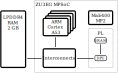
\includegraphics[width=0.5\textwidth]{graphics/hardware_overview.pdf}
	\caption{Available hardware on the Ultra96-V2}
	\label{fig:hardware_overview}
\end{figure}

\section{Camera Library}
\label{sec:inference:camera_library}
\todo[inline]{not done yet}



\section{Package}
\label{sec:inference:package}

Both the inference application and the Python scripts used during training require a lot of similar functionality (e.g. settings, constants, database connectivity).
For this reason the \texttt{fhnwtoys} Python package, consisting of several modules (\texttt{.py} files), was created.

\subsection{Structure}
\label{subsec:inference:package:structure}
There are three main modules:
\begin{enumerate}
  \item Definitions (\texttt{definitions.py})
  \item Settings (\texttt{settings.py})
  \item Enums (\texttt{enums.py})
\end{enumerate}

The \texttt{fhnwtoys.definitions} module contains, as the name suggests, several definitions (functions and classes).
These definitions are only used during the training and verification process on the host.

The \texttt{fhnwtoys.settings} module contains various names and settings that are used throughout the project (e.g. the names of the objects, file names, camera settings).

The \texttt{fhnwtoys.enums} module contains a bunch of enumerations which provide a convenient way to work with a set of related constants \cite{inf_enum}.
This improves the readability of the code by removing magic numbers (unexplained numerical constants).

Additionally, there are two modules that can be used to import the required main modules:
\begin{enumerate}
  \item Training (\texttt{training.py})
  \item Inference (\texttt{inference.py})
\end{enumerate}

Importing the \texttt{fhnwtoys.training} module provides access to all three main modules.

Importing the \texttt{fhnwtoys.inference} module is the same as importing the \texttt{fhnwtoys} package directly, as it is an alias for the \texttt{fhnwtoys.\_\_init\_\_} module.
However, explicitly importing the \texttt{fhnwtoys.inference} module is the preferred method.
This provides acces to the \texttt{fhnwtoys.settings} and \texttt{fhnwtoys.enums} modules.

% --------------------------------
\subsection{Importing the Package}
\label{subsec:inference:package:importing_the_package}
Listing \ref{lst:importing_package} shows how to import the \texttt{fhnwtoys} package.
For convenience purposes, the imported package is aliased as \texttt{fh}.

\begin{lstlisting}[style=python, caption={Importing the \texttt{fhnwtoys} Python package}, label=lst:importing_package]
import fhnwtoys.training as fh # training and verification
import fhnwtoys.inference as fh # inference application
\end{lstlisting}

% -----------------------
\subsection{Installation}
\label{subsec:inference:package:installation}
A setup script is provided which allows for an easy installation of the \texttt{fhnwtoys} package.
It can be installed with the following command from the \texttt{packages/} directory:

\begin{lstlisting}[style=bash]
sudo pip3 install -e .
\end{lstlisting}

\section{User Interface}
\label{sec:inference:user_interface}

The \acrfull{ui} is designed to be simple and modern.
It features two different layouts: a bootsplash screen and an inference screen.
The bootsplash screen shows information about the boot process (e.g. initialization messages, error messages) and the inference screen shows the classification results of the latest throw.
No user input is required, as the application is almost immediately ready again after displaying the results of the latest throw.

% ------------------------------------------------------------------------------------------------------------------------------
\subsection{Bootsplash Screen}
\label{subsec:inference:user_interface:bootsplash_screen}

The bootsplash screen is displayed during the initialization phase of the application.
It consists of the FHNW logo in the top left corner, the title of the project, the names of the project authors and a configurable status message.
The configurable status message is used to display both initialization messages and camera error messages.

A bootsplash screen with an initialization status message is shown in figure \ref{fig:ui_boot}.

\begin{figure}
  \centering
  \includegraphics[width=\textwidth]{ui/ui_boot}
  \caption{Bootsplash screen with a camera initialization message}
  \label{fig:ui_boot}
\end{figure}

% ------------------------------------------------------------------------------------------------------------------------------
\subsection{Inference Screen}
\label{subsec:inference:user_interface:inference_screen}

The inference screen is displayed after a detected throw has been evaluated.
It consists of the FHNW logo in the top left corner, an acquired image of the object on the left half of the screen and the classification statistics on the right half of the screen.

The displayed image of the object is the one with the highest weighted prediction percentage of the class selected as the best prediction.
This is most likely a frame from the middle of the throw due to the applied weighting (see section \ref{subsec:inference:app:ui}).

The classification statistics are visualized in a donut chart which shows the best prediction, up to three additional predictions and the sum of the rest of the prediction percentages.
Additional predictions are only shown if their percentages are greater or equal to \SI{1.0}{\percent}.
Furthermore, the sum of the rest of the percentages is only shown if it is not equal to zero after rounding.
All percentages are rounded to one decimal place before being displayed (see section \ref{subsec:inference:app:ui}).

Displaying the throughput of the image classification chain in frames per second is not necessary as it remains more or less constant.
The small differences are due to background tasks of the Linux operating system (see section \ref{sec:verification_and_benchmark:throughput}).

Figure \ref{fig:ui_inference_paper_ball} show an example of the inference screen.
The classification accuracy, however, reaches \SI{100.0}{\percent} in most cases.
Therefore, the inference screen usually looks more like the one shown in figure \ref{fig:ui_inference_bunny}.

\begin{figure}
  \centering
  \includegraphics[width=\textwidth]{ui/ui_inference_paper_ball}
  \caption{Example of an inference screen showing the \textit{Paper Ball}}
  \label{fig:ui_inference_paper_ball}
\end{figure}

\begin{figure}
  \centering
  \includegraphics[width=\textwidth]{ui/ui_inference_bunny}
  \caption{Example of an inference screen with a prediction of \SI{100.0}{\percent}}
  \label{fig:ui_inference_bunny}
\end{figure}

% ------------------------------------------------------------------------------------------------------------------------------
\subsection{Implementation}
\label{subsec:inference:user_interface:implementation}

The \acrlong{ui} is implemented as a class in the Python module \texttt{ui.py} and uses the Python packages PySimpleGUI as well as Matplotlib.

PySimpleGUI allows for the creation of simple \acrlongpl{ui} that work across multiple platforms.
Currently, there exist four ports of PySimpleGUI and the Tkinter variant is used by default \cite{inf_pysimplegui}.
Tkinter is the standard Python interface to the Tk cross-platform widget toolkit that provides a library of graphical widgets to build \acrlongpl{ui} \cite{inf_tkinter}.

Matplotlib is a flexible plotting library which provides a MATLAB-like interface with the \texttt{pyplot} module.
Even though it is extremely easy to use, full control over the various properties is not sacrificed as low-level commands are also available \cite{inf_matplotlib}.

% ------------------------------
\paragraph{User Interface Class}
The \texttt{UI} class consists of several non-blocking methods to update the \acrlong{ui} screens.
Calling the PySimpleGUI \texttt{read} method of the \texttt{Window} class is used to update the screens.
However, this call blocks the Python interpreter until a user event occurs (e.g. a button click).
This standard \acrlong{ui} behaviour would render the entire package unusable.
Fortunately, the \texttt{read} method allows to specify a timeout, which essentially turns it into polling mode.
It is therefore called with a short timeout of \SI{100}{ms}, which is necessary to update the screen \cite{inf_pysimplegui_ref}.

The \texttt{boot\_window} and \texttt{inference\_window} methods are used to spawn windows with the appropriate layouts described in section \ref{subsec:inference:user_interface:bootsplash_screen} and \ref{subsec:inference:user_interface:inference_screen}.

The main methods are \texttt{update\_boot\_window} and \texttt{update\_inference\_window}.
When called, they first check whether the screen layout is set to the requested one and switch to it if necessary.
The \acrlong{ui} screen is then updated in a second step and requires the status message in case of the bootsplash screen.
Updating the inference screen requires a list of the predictions, a list of the prediction percentages and the \acrshort{png} encoded image data.

% -----------------------------------
\paragraph{Classification Statistics}
The \texttt{figure} method uses Matplotlib to turn the classification statistics into a donut chart.
Directly generating a donut chart is, however, not possible with Matplotlib.
Therefore, a circle with the same color as the background is placed in the middle of a pie chart.
This simple modification creates the desired donut chart.

To display the figure on the screen, it must be in the \acrshort{png} file format.
For this reason, it is saved to an in-memory \texttt{bytes} buffer to avoid slow file operations.
This is implemented in the \texttt{get\_img\_from\_figure} method.

Animating the ring of the donut chart with Matplotlib would easily be possible by rendering several versions of it overlaid with a circular sector in the background color.
As time passes, the central angle of the circular sector is decreased, starting at the top of the ring and progressing in a clockwise direction around the ring.
This would give the appearance that the ring is being drawn on the display.
Unfortunately, the processor of the embedded system is not powerful enough to render several versions of the donut chart in a reasonable amount of time.

% ----------------
\paragraph{Cursor}
The cursor cannot be disabled globally, but it is possible to hide it when it is hovering over certain elements (e.g. text, images).
For this purpose, the underlying Tkinter widgets are accessed with the \texttt{Widget} class variable and the cursor is set to invisible \cite{inf_pysimplegui_widget}.
The cursor position is centered on the screen after booting.
Therefore, the respective Tkinter widgets located in the center are modified to hide the cursor.

\section{Application}
\label{sec:inference:app}
% \todo[inline]{entire code in appendix? => Yes, todos, cleanup}
% \todo[inline]{write that row vectors are meant if not specified otherwise? => probably not necessary, easily spottable due to the context}

The inference application is written in Python 3 and the complete listing can be found in appendix \ref{app:inference_application}.
% Although Python is not known for extremely fast execution times there are several tricks which make it possible to run almost as fast as a native app.
% Although Python is not known for extremely fast execution times, there are some tricks that allow it to run almost as fast as a native application.
Although Python is not known for extremely fast execution times, it allows for fast and easy development.
% Furthermore, several methods are used that allow the inference application to run almost as fast as a native application.
Furthermore, several methods are used to improve the speed of execution.
This allows the inference application to run almost as fast as a native application.
% Additionally

% overview (not a chapter)
% routine of the app
% 1. init cam / 2. ...
% This section explains the procedure of the inference application shown in figure \ref{fig:procedure_inference_app}.
This section describes the procedure of the inference application shown in figure \ref{fig:procedure_inference_app}.
% After the initialization of the \acrshort{dpu} and the camera, the frame acquisition is stared.
After the initialization of the \acrshort{dpu} and the camera, the image acquisition is stared.
% Once a throw has been detected
Once a throw has been completed, the frames are processed and several predictions are made.
These predictions are then weighted and the result is displayed on the screen.
% Lastly, the global variables are reset and the image acquisition is started again.
% In a last step, the global variables are reset to their original values.
Finally, the global variables are reset to their original values.
% This completes the cycle and the image acquisition is started again.
This completes the sequence and the image acquisition is started again.
This completes the never-ending sequence and the image acquisition is started again.

\begin{figure}
  \centering
  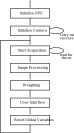
\includegraphics[width=0.5\textwidth]{program_flow} % done: draw and add procedure graphics
  \caption{Procedure of the inference application}
  \label{fig:procedure_inference_app}
\end{figure}

% ------------------------------------------------------------------------------------------------------------------------------
\subsection{Initialization}
\label{subsec:inference:app:initialization}
\todo[inline]{not done yet}

% init DPU
% done with overlays
% (thin wrapper around N2Cube)

% loads the overlay (architecture ad weights of the neural network)

% explain those two:
% from dnndk import n2cube
% from pynq_dpu import DpuOverlay



% Camera
% init camera
% - wait until successful (show error in the UI)
% start acquisition
% - multi processing
% reset variables
% terminate




% ------------------------------------------------------------------------------------------------------------------------------
\subsection{Image Acquisition}
\label{subsec:inference:app:image_acquisition}
\todo[inline]{not done yet}



% explain import ctypes shortly

% explain that this is used:
% from threading import Thread








% ## our application

% - explain how it could have been done in C++ or Python
%   - python wins, because it's easier for quick prototyping
%   - there is no (noticable) performance loss when using Python, since the same N2Cube lib is used with a minimal Python wrapper around it (this is possible with ctypes, since cpython is used [most common])
%     - there is also no perfomance loss for the camera application because of the same reason (ctypes-implementation)
%   - explain both processes in detail (C++ with the CMake file, which requires the sysroot with all the headers and shared objects [libraries])
%     - maybe talk about the docker conatainer which could be used but is not ideal if you add stuff to the sysroot, weh creating your own PwtaLinux with opencv + baumer...
%   - explain that the C++ and Python API are very similar and so a conversion between the two is not really difficult






















% ------------------------------------------------------------------------------------------------------------------------------
\subsection{Image Processing}
\label{subsec:inference:app:image_processing}
\todo[inline]{not finished yet}


% ----------------------------------------------------
\paragraph{Empirical Cumulative Distribution Function}
% plot that shows with 22 frames everything is good
% Histogram (Bimodal) => no, a histogram is used for continuous data!
% Figure \ref{fig:frame_distribution} shows the distribution of the number of frames per throw $f(n)$.
% The distribution of the number of frames per throw $f(x)$ is shown in figure \ref{fig:frame_distribution}.
% The distribution of the number of throws with $x$ frames $f(x)$ is shown in figure \ref{fig:frame_distribution}.
% The distribution of the number of frames per throw $f(x)$ is shown in figure \ref{fig:distribution}.
The empirical distribution of the number of frames per throw $f(x)$ is shown in figure \ref{fig:distribution}.
% The normalized summation of the frame distribution $F(n)$ is calculated with the following equation:
% Figure \ref{fig:frame_distribution_summation} shows the normalized summation of the frame distribution $F(n)$, which can be calculated with equation \ref{eq:frame_distribution_summation}.
% The empirical distribution function
% The discrete cumulative distribution function of
% The empirical cumulative distribution function of
% Figure \ref{fig:frame_distribution_summation} shows the empirical cumulative distribution function $F(n)$, which can be calculated with equation \ref{eq:frame_distribution_summation}.
% Figure \ref{fig:cumulative_distribution} shows the empirical cumulative distribution function $F(x)$, which can
% Figure \ref{fig:cumulative_distribution} shows the empirical cumulative distribution function $F(x)$ of the distribution $f(x)$.
This distribution is used to derive the empirical cumulative distribution function $F(x)$ shown in figure \ref{fig:cumulative_distribution}.

\begin{figure}
  \centering
  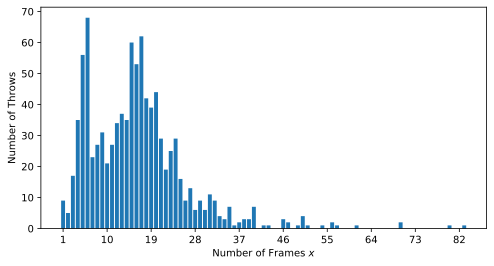
\includegraphics[width=\textwidth]{distribution}
  \caption{Distribution of the number of frames per throw $f(n)$}
  \label{fig:distribution}
\end{figure}

\begin{figure}
  \centering
  \includegraphics[width=\textwidth]{cumulative_distribution}
  % \caption{Normalized summation of the frame distribution $F(n)$}
  \caption{Empirical cumulative distribution function $F(x)$}
  \label{fig:cumulative_distribution}
\end{figure}

% \begin{equation}
%   F(n) = \sum\limits_{i=1}^{n} f(i)
%   \label{eq:frame_distribution_summation}
% \end{equation}



% explain that those are used:
% import cv2
% import numpy as np


% resizing, ...
\begin{enumerate}
  \item Getting the raw Baumer BayerRG8 frame
  \item Converting the color space
  \item Resizing the frame
  \item Normalizing the pixel values
  \item Running inference
\end{enumerate}


% ---------------------------
\paragraph{Running Inference}
% explain the calls to run inference

% these are the output values of the CNN (from the output layer)
% The output values $\boldsymbol{z}$ of the \acrshort{cnn} model
The output values of the \acrshort{cnn} model are denoted by the output vector

\begin{equation}
  \boldsymbol{z} =
  \begin{bmatrix}
    z_1 & z_2 & \dots & z_c \\
  \end{bmatrix}.
  \label{eq:output_vector}
\end{equation}

The values of the output vector $\boldsymbol{z}$ are 8-bit integers which represent a fixed-point format.
% on these the softmax function is used to get probabilities (read more theory about this!)
% To normalize the the output vector to a probability distribution, the softmax function is used.
The softmax function is used to normalize the values of the output vector to a discrete probability distribution over the target classes.
% formula for softmax!

% todo: cite https://towardsdatascience.com/softmax-activation-function-explained-a7e1bc3ad60
% todo: or maybe cite this https://towardsdatascience.com/the-softmax-function-neural-net-outputs-as-probabilities-and-ensemble-classifiers-9bd94d75932


\begin{equation}
  p_k = \frac{e^{z_k}}{\sum\limits_{i=1}^{c} e^{z_i}}
  \label{eq:softmax}
\end{equation}

where

\[
  % 1\leq k\leq c
  k = 1, 2, \dots, c
\]

and

\begin{tabular}{lll}
  $p_k$ & = & probability $k$ of the prediction vector $\boldsymbol{p}$ \\
  $z_k$ & = & output value $k$ of output vector $\boldsymbol{z}$ \\
  $c$ & = & number of classes \\
  $z_i$ & = & output value $i$ of output vector $\boldsymbol{z}$ \\
\end{tabular}
\\



% implementation with n2cube


% adding the individual probabilities to an array
% this essentailly creates the prediction vector p
% results in the prediction vector p

% prediction vector p

\begin{equation}
  \boldsymbol{p} =
  \begin{bmatrix}
    p_1 & p_2 & \dots & p_c \\
  \end{bmatrix}
  \label{eq:prediction_vector}
\end{equation}




% the individual predictions are added to an array
% this essentially creates the predictions matrix

% predictions matrix P

\begin{equation}
  \boldsymbol{P} =
  \begin{bmatrix}
    \boldsymbol{p}_1 \\
    \boldsymbol{p}_2 \\
    \vdots \\
    \boldsymbol{p}_n \\
  \end{bmatrix} =
  \begin{bmatrix}
    P_{11} & P_{12} & \dots & P_{1c} \\
    P_{21} & P_{22} & \dots & P_{2c} \\
    \vdots & \vdots & \ddots & \vdots \\
    P_{n1} & P_{n2} & \dots & P_{nc} \\
  \end{bmatrix}
  \label{eq:predictions_matrix}
\end{equation}




% NaN detection and fix









% ------------------------------------------------------------------------------------------------------------------------------
\subsection{Weighting}
\label{subsec:inference:app:weighting}

% The verification of the classification accuracy has shown that images, where the object is fully visible on the frame, perform significantly better than frames, where the object is only partially visible (see section \ref{sec:training}). % todo: add correct reference
Verifying the classification accuracy has shown that images in which the object is fully visible perform significantly better than frames in which the object is only partially visible (see section \ref{subsec:verification_and_benchmark:classification_performance:inference}). % todo: add correct reference
% For this reason, a discrete weighting function is applied to the predictions.
For this reason, a discrete sine-squared weighting function is applied to the predictions.
% For this reason, the stretched and phase-shifted sine-squared window function is applied.
% sine squared discrete window function (explain why not sine => or do not)
% To give more importance to frames from the middle of the throw, a stretched and phase-shifted sine-squared window function is used.
% To give more importance to frames from the middle of the throw, a discrete sine-squared window function is used.

% --------------------------
\paragraph{Number of Frames}
% To properly weight the predictions, not only the number of frames considered $n$ but also the total number of frames $N$ is important.
To properly weight the predictions, not only the number of frames considered $n$ is important, but also the total number of frames $N$.
% number of frames considered $n$ vs. the total number of frames $N$
The relationship between the two is given in equation \ref{eq:number_of_frames}.
Not considering the total number of frames would implicitly assume that the throw was only \num{22} frames long.
% If the total number of frames would not to be considered,
Throws of larger objects, which generally create more frames, would then be incorrectly weighted.
Furthermore, knowing if the throw created more than \num{44} frames is not really beneficial because of the symmetry of the weighting function.
% This information would only really matter if the total number of frames could get extremely large, which it cannot.
This information would only be relevant if the total number of frames could get extremely large, which it cannot.

\begin{equation}
  n =
  \begin{cases}
    N & N \leq 22 \\
    % M_{i,j}^{k} + \Delta & 0\leq M_{i,j}^{k} + \Delta\leq 255 \\
    22 & N > 22 \\
  \end{cases}
  \label{eq:number_of_frames}
\end{equation}

where

\begin{tabular}{lll}
  $n$ & = & number of frames considered \\
  $N$ & = & total number of frames \\
\end{tabular}
\\

% ----------------------------
\paragraph{Weighting Function}
% The employed weighting function is the discrete version of a stretched and phase-shifted sine-squared window function.
% stretched and phase-shifted sine-squared discrete window function
The used weighting function is the discrete version of a stretched and phase-shifted sine-squared window function.
% weights can be calculated
The individual weights can be calculated with equation \ref{eq:weighting_function}.
An example of the discrete weighting function with $n = 22$ and $N = 28$ is shown in figure \ref{fig:weighting_function}.

\begin{equation}
  % w_k = \sin^2\left(\frac{k+1}{N+1} \cdot \pi \right)
  w_k = \sin^2\left(\frac{k}{N+1} \cdot \pi \right)
  \label{eq:weighting_function}
\end{equation}

where

\[
  % 1\leq k\leq n
  k = 1, 2, \dots, n
\]

and

\begin{tabular}{lll}
  $w_k$ & = & weighting factor $k$ of the weight vector $\boldsymbol{w}$ \\
  $N$ & = & total number of frames \\
  $n$ & = & number of frames considered \\
\end{tabular}
\\

\begin{figure}
  \centering
  \includegraphics[width=\textwidth]{weighting_function}
  \caption{Weighting function with $n = 22$ and $N = 28$}
  \label{fig:weighting_function}
\end{figure}

% results in the weight vector w
This results in the weight vector
\begin{equation}
  \boldsymbol{w} =
  \begin{bmatrix}
    w_{1} & w_{2} & \dots & w_{n} \\
  \end{bmatrix}.
  \label{eq:weight_vector}
\end{equation}

% talk about the implementation (constant size array filed with zero)
% talk about that always the maximum amount of frames considered weights is returned (the rest is filled with zeros)
% This results in the following weight vector with $n$ elements: % $\boldsymbol{w}$
The weight vector is implemented as a fixed size one-dimensional NumPy array. % of type \texttt{np.float32}.
% The length of this array is equal to the maximum number of frames to consider, which is \num{22}.
The length of this array corresponds to the maximum number of frames to be considered, which is \num{22}.
If a throw creates less than \num{22} frames, the rest of the array is filled with zeros.
% The window function is implemented in the \texttt{sine\_squared\_window} function 
This is implemented in the \texttt{sine\_squared\_window} function, as shown in appendix \ref{app:inference_application} on line \ref{lst:ln:sine_squared_window}.

% --------------------------------------
\paragraph{Weighting of the Predictions} % Probabilities
% predictions are then weighted (reference to verificcation that shows that partial throws perform worse than fully visible ones)
% weighted average
The individual probabilities are weighted according to equation \ref{eq:weighted_probability}.

\begin{equation}
  y_k = \frac{w_1 \cdot P_{1k} + w_2 \cdot P_{2k} + \dots + w_n \cdot P_{nk}}{w_1 + w_2 + \dots + w_n} = \frac{\sum\limits_{i=1}^{n} w_i \cdot P_{ik}}{\sum\limits_{i=1}^{n} w_i}
  \label{eq:weighted_probability}
\end{equation}

where

\[
  % 1\leq k\leq c
  k = 1, 2, \dots, c
\]

and

\begin{tabular}{lll}
  $y_k$ & = & weighted probability $k$ of the weighted prediction vector $\boldsymbol{y}$ \\ % prediction
  $w_i$ & = & weighting factor $i$ of the weight vector $\boldsymbol{w}$ \\
  $P_{i,k}$ & = & probability $i,k$ of the predictions matrix $\boldsymbol{P}$ \\
  $n$ & = & number of frames considered \\
  $c$ & = & number of classes \\
\end{tabular}
\\

This results in the weighted prediction vector
\begin{equation}
  \boldsymbol{y} =
  \begin{bmatrix}
    y_{1} & y_{2} & \dots & y_{n} \\
  \end{bmatrix}.
  \label{eq:weighted_prediction_vector}
\end{equation}

% this can also be done with matrix multiplication
% done with numpy, explain the implementation and reference to it
% The actual implementation uses matrix multiplication to simplify equation \ref{eq:weighted_probability}.
The actual implementation uses matrix multiplication to perform this calculation efficiently.
Therefore, the NumPy function \texttt{np.matmul} is used to calculate the matrix product of the two arrays \cite{}. % todo: cite https://numpy.org/doc/stable/reference/generated/numpy.matmul.html
This is shown in appendix \ref{app:inference_application} on line \ref{lst:ln:matrix_multiplication}.

% todo: which version should be used?
% todo: \cdot between matrix multiplication? -> No, could be misinterpreted as the dot product
\begin{equation}
  % \boldsymbol{y} = \sum\limits_{i=1}^{n} \frac{1}{w_i} \cdot \boldsymbol{w} \boldsymbol{P}
  \boldsymbol{y} = \sum\limits_{i=1}^{n} w_i^{-1} \cdot \boldsymbol{w} \boldsymbol{P}
  \label{eq:weighted_prediction}
\end{equation}

where

\begin{tabular}{lll}
  $\boldsymbol{y}$ & = & weighted prediction vector \\ % of length $c$
  $n$ & = & number of frames considered \\
  $w_i$ & = & weighting factor $i$ of the weight vector $\boldsymbol{w}$ \\
  $\boldsymbol{w}$ & = & weight vector \\ % of length $n$
  $\boldsymbol{P}$ & = & predictions matrix \\ % $n \times c$
\end{tabular}
\\

% ------------------------------------------------------------------------------------------------------------------------------
\subsection{User Interface}
\label{subsec:inference:app:ui}
% show results (UI)

% To display the results on the screen, they have to be prepared
% The results have to be prepared to be displayed on the screen.
The results must be prepared to be displayed on the screen.
% On the one hand, a suitable frame of the throw has to be selected and on the other hand the probabilities have to be rounded
On the one hand, an appropriate frame of the captured throw has to be selected and, on the other hand, the probabilities have to be rounded and prepared in a list.

% -------------------------
\paragraph{Frame Selection}
% weighting of the frames to chose the best frame
Choosing an appropriate frame of the captured throw is done by selecting the image with the highest weighted probability of the class selected as the best prediction. % prediction made by the model
% The image with the highest weighted probability of the class selected as the best prediction is chosen.
% This corresponds to weighting the respective column of the predictions matrix $\boldsymbol{P}$, which is shown in equation \ref{eq:weighted_probabilities}.
% For this purpose the weight column vector $\boldsymbol{w}^\top$ is element-wise multiplied with 
% For this purpose, the weighted probabilities column vector $\boldsymbol{f}$ is calculated as shown in equation \ref{eq:weighted_probabilities}.
% This corresponds to the element-wise multiplication of the weight column vector $\boldsymbol{w}^\top$ with the respective column of the predictions matrix $\boldsymbol{P}$, which is shown in equation \ref{eq:weighted_probabilities}.
% For this purpose, the element-wise multiplication of the weight column vector $\boldsymbol{w}^\top$ with the respective column of the predictions matrix $\boldsymbol{P}$ is calculated, which is shown in equation \ref{eq:weighted_probabilities}.
For this purpose, the element-wise multiplication of the weight column vector $\boldsymbol{w}^\top$ with the respective column of the predictions matrix $\boldsymbol{P}$ is calculated.
This is shown in equation \ref{eq:weighted_probabilities}.
The image corresponding to the index of the highest weighted probability is then selected.
% The image corresponding to the index of the highest weighted probability, which is most likely a frame from the middle of the throw, is then selected.
% This is most likely a frame from the middle of the throw due to the applied weighting.
Due to the applied weighting, this is most likely a frame from the middle of the throw, where the object is most visible.

% todo: maybe use \odot
\begin{equation}
  \boldsymbol{f} = \boldsymbol{w}^\top \circ \boldsymbol{P}_{:,k} =
  \begin{bmatrix}
    w_{1} \cdot P_{1,k} \\
    w_{2} \cdot P_{2,k} \\
    \vdots \\
    w_{n} \cdot P_{n,k} \\
  \end{bmatrix}
  \label{eq:weighted_probabilities}
\end{equation}

where

\begin{tabular}{lll}
  $\boldsymbol{f}$ & = & weighted probabilities column vector \\
  $\boldsymbol{w}^\top$ & = & weight column vector \\
  $\boldsymbol{P}_{:,k}$ & = & column $k$ of the predictions matrix $\boldsymbol{P}$ \\
  $w_i$ & = & weighting factor $i$ of the weight vector $\boldsymbol{w}$ \\
  $P_{i,k}$ & = & probability $i,k$ of the predictions matrix $\boldsymbol{P}$ \\
  $n$ & = & number of frames considered \\
\end{tabular}
\\

The frame is then resized and encoded as a \acrshort{png}.
The implementation of the image selection and preparation process is shown in appendix \ref{app:inference_application} on lines \ref{lst:ln:frame_selection1}--\ref{lst:ln:frame_selection2}.

% ---------------------------------------
\paragraph{Rounding of the Probabilities}
% lrm round function
% The percentages are rounded to one decimal place.
% Before displaying the probabilities, they are rounded to one decimal place.
The probabilities (in percent) are rounded to one decimal place before they are displayed on the screen.
However, naively rounding percentages will quickly reveal the problem that the total value does not always add up to \SI{100}{\percent}.
The largest remainder method is used to fix this problem.
This simple method consists of the following easy three steps \cite{}: % todo: cite https://revs.runtime-revolution.com/getting-100-with-rounded-percentages-273ffa70252b
\begin{enumerate}
  \item Flooring all values
  % \item Computing the difference between the sum of the floored values and the total value
  \item Computing the difference between the total value and the sum of the floored values
  % \item Distributing this difference by adding one to each floored value until
  % \item Distributing this difference by adding one to each floored value in decreasing order of their decimal parts
  % \item Distributing the difference between the floored values in decreasing order of their decimal parts
  \item Distributing this difference by incrementing the floored values in decreasing order of their decimal parts
\end{enumerate}

% Listing \ref{lst:largest_remainder_method} shows the implementation of the largest remainder method in the \texttt{lrm\_round} function.
The largest remainder method is implemented in the \texttt{lrm\_round} function, as shown in appendix \ref{app:inference_application} on line \ref{lst:ln:lrm_round}. % done: maybe reference to appendix line xyz instead of another listing of this function?
% To round the percentages to one decimal place, the values are multiplied by ten and \num{1000} is used as the total value.
To round the percentages to one decimal place, the values are multiplied by ten before the algorithm is applied.
% As a last step, the values are divided by ten which results in percentages rounded to one decimal place.
In a final step, the values are divided by ten, resulting in percentages rounded to one decimal place.

% \begin{lstlisting}[style=python, caption={Largest remainder method}, label=lst:largest_remainder_method]
% def lrm_round(series):
%   floored_series = np.floor(series * 10.0)
%   decimal_series = series * 10.0 - floored_series
%   decimal_series_argsorted = np.argsort(decimal_series)[::-1]
%   difference = 1000 - np.sum(floored_series, dtype=np.uint16)
%   for idx in decimal_series_argsorted[0:difference]:
%     floored_series[idx] += 1
%   return_series = floored_series.astype(np.float64) / 10.0
%   return return_series.tolist()
% \end{lstlisting}

